% AVA PyTICS ensemble workflow (ava.photometry.ensemble + intercal), Nov 2026.
% Standalone: `latexmk -pdf pytics_workflow.tex` -> pytics_workflow.pdf; in the manual
% \includegraphics[width=\textwidth]{figures/pytics/pytics_workflow.pdf}
% Grey boxes = published PyTICS (Vieliute et al. 2025, Filter.Corr), orange = AVA changes/additions.
\documentclass[tikz,border=6pt]{standalone}
\usepackage[T1]{fontenc}
\usepackage{lmodern}
\usepackage{amsmath}
\pagecolor{white}
\usetikzlibrary{positioning,arrows.meta,fit,backgrounds,calc,shapes.geometric}

\definecolor{orig}{HTML}{E9EEF3}
\definecolor{origline}{HTML}{4A6274}
\definecolor{ava}{HTML}{FDE6CC}
\definecolor{avaline}{HTML}{C0661A}
\definecolor{io}{HTML}{E4F1E4}
\definecolor{ioline}{HTML}{3D7A3D}

\tikzset{
  box/.style={draw=origline, fill=orig, rounded corners=2pt, align=left, font=\footnotesize,
              text width=#1, inner sep=4pt, line width=0.6pt},
  box/.default=7.2cm,
  ava/.style={box=#1, draw=avaline, fill=ava},
  ava/.default=7.2cm,
  io/.style={box=#1, draw=ioline, fill=io},
  io/.default=7.2cm,
  dec/.style={draw=origline, fill=white, diamond, aspect=2.6, align=center, font=\footnotesize, inner sep=1pt},
  arr/.style={-{Stealth[length=5pt]}, line width=0.7pt, draw=black!70},
  lab/.style={font=\scriptsize\itshape, text=black!70},
  tag/.style={font=\scriptsize\bfseries, text=avaline},
}

\begin{document}
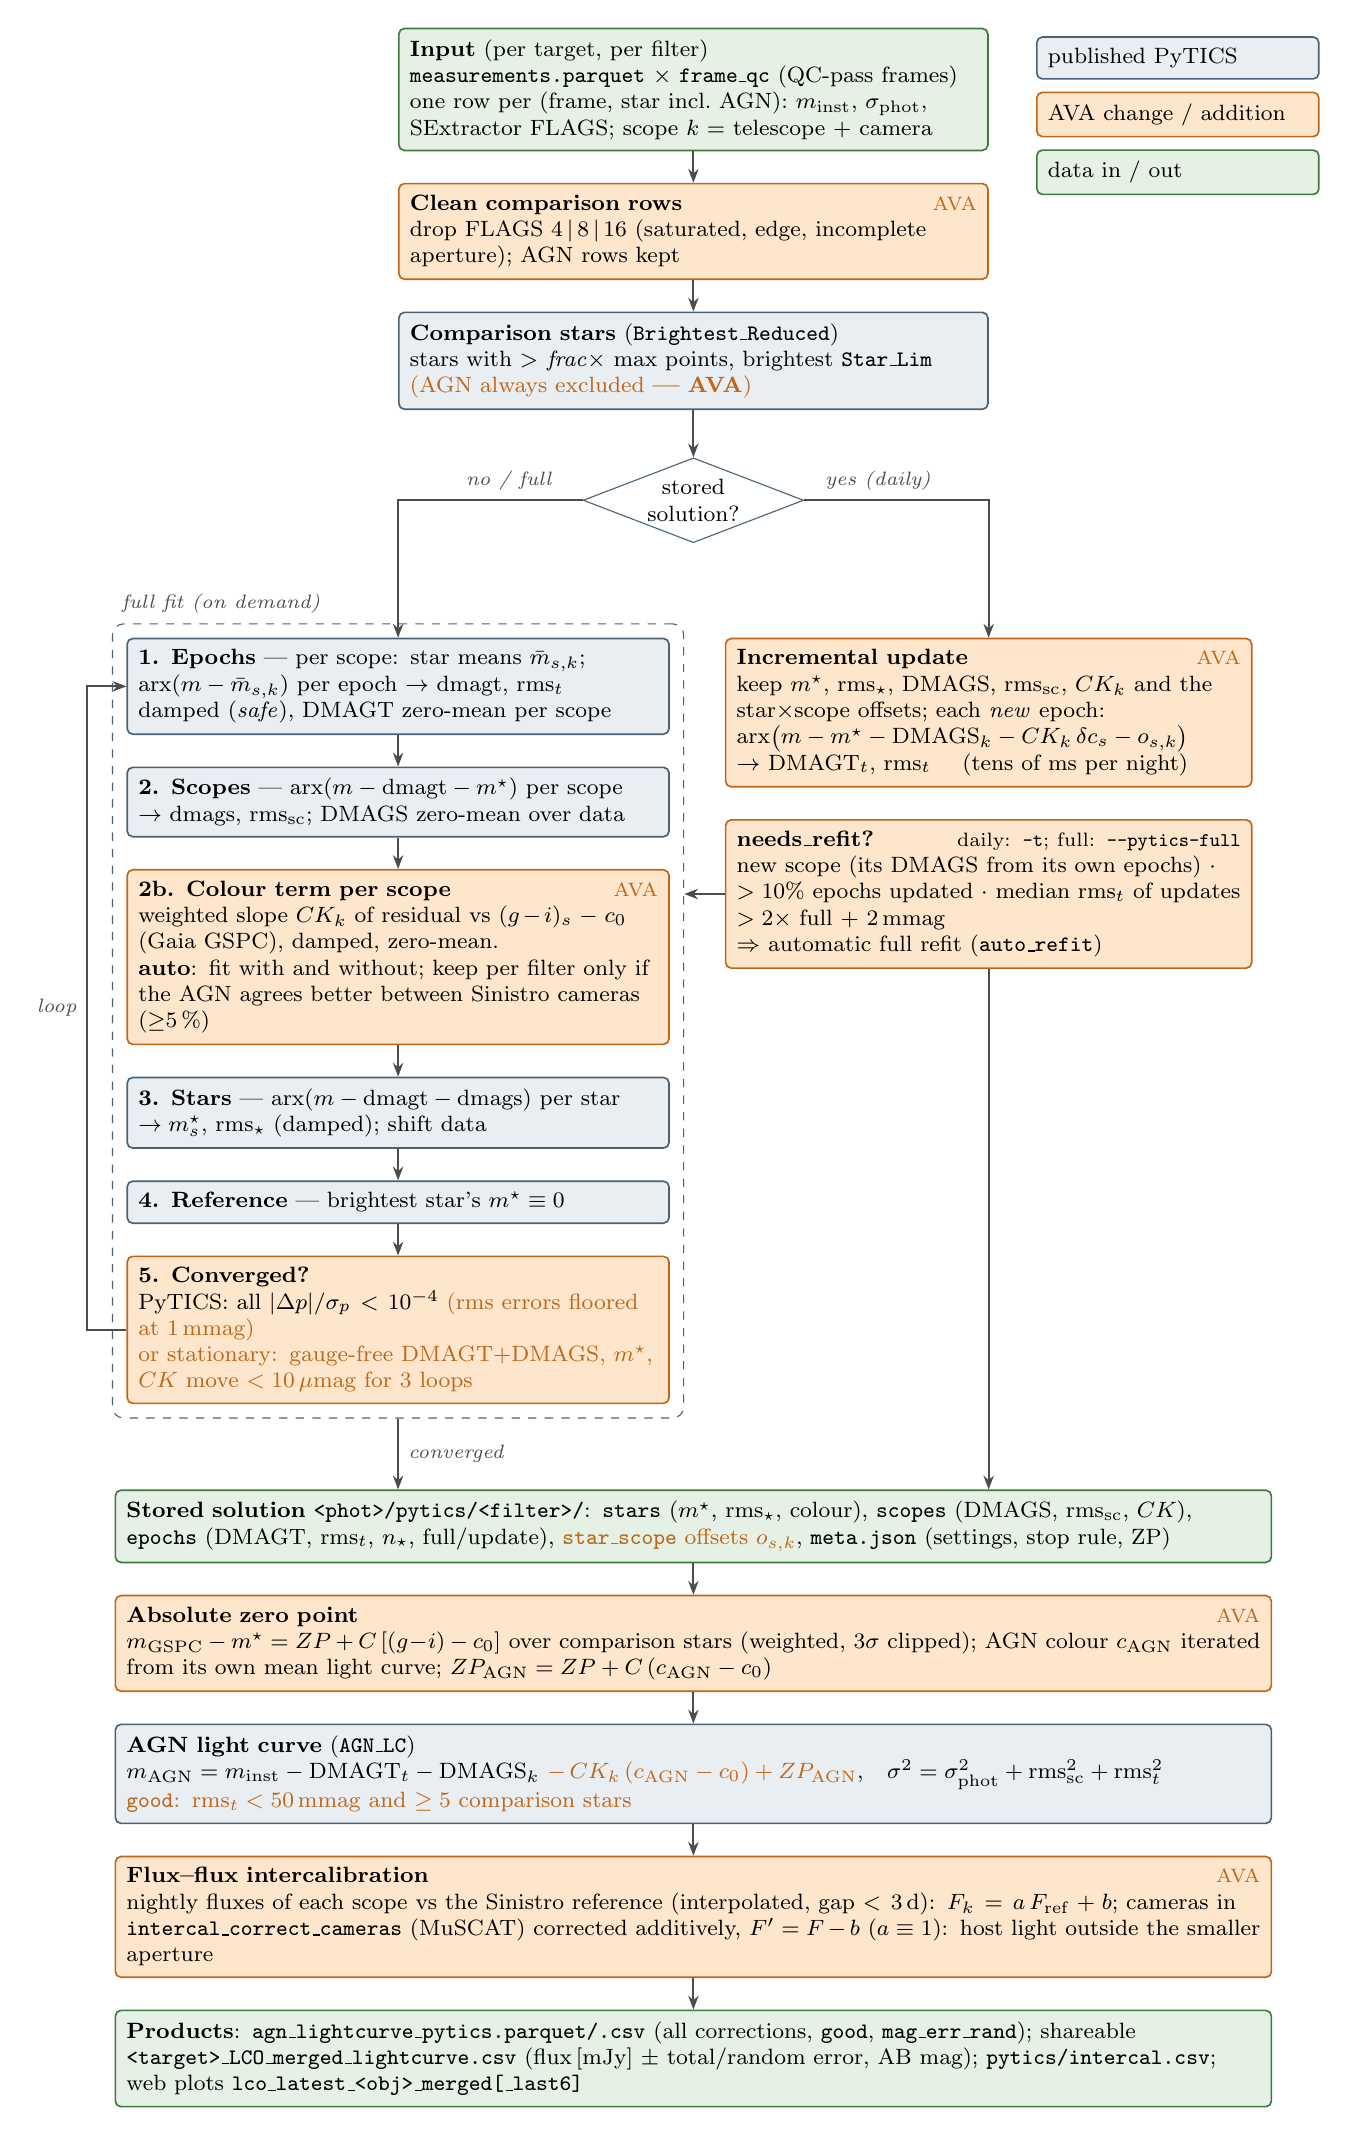
\begin{tikzpicture}[node distance=4mm]

% ---------------- inputs ----------------
\node[io] (in) {\textbf{Input} (per target, per filter)\\
  \texttt{measurements.parquet} $\times$ \texttt{frame\_qc} (QC-pass frames)\\
  one row per (frame, star incl.\ AGN): $m_\mathrm{inst}$, $\sigma_\mathrm{phot}$, SExtractor FLAGS;
  scope $k$ = telescope + camera};

\node[ava, below=of in] (clean) {\textbf{Clean comparison rows} \hfill\textcolor{avaline}{\scriptsize AVA}\\
  drop FLAGS $4\,|\,8\,|\,16$ (saturated, edge, incomplete aperture); AGN rows kept};

\node[box, below=of clean] (sel) {\textbf{Comparison stars} (\texttt{Brightest\_Reduced})\\
  stars with $>\!\mathit{frac}\times$ max points, brightest \texttt{Star\_Lim}
  \textcolor{avaline}{(AGN always excluded \textbf{--- AVA})}};

\node[dec, below=6mm of sel] (mode) {stored\\solution?};

% ---------------- full fit (left) ----------------
\node[box=6.6cm, below=12mm of mode, xshift=-3.75cm] (s1) {\textbf{1. Epochs} --- per scope: star means $\bar m_{s,k}$;\\
  $\mathrm{arx}(m - \bar m_{s,k})$ per epoch $\to$ dmagt, rms$_t$\\
  damped ($\mathit{safe}$), DMAGT zero-mean per scope};
\node[box=6.6cm, below=of s1] (s2) {\textbf{2. Scopes} --- $\mathrm{arx}(m - \mathrm{dmagt} - m^\star)$ per scope\\
  $\to$ dmags, rms$_\mathrm{sc}$; DMAGS zero-mean over data};
\node[ava=6.6cm, below=of s2] (s2b) {\textbf{2b. Colour term per scope} \hfill\textcolor{avaline}{\scriptsize AVA}\\
  weighted slope $CK_k$ of residual vs $(g\!-\!i)_s - c_0$ (Gaia GSPC), damped, zero-mean.\\
  \textbf{auto}: fit with and without; keep per filter only if the AGN agrees better between Sinistro cameras ($\ge$5\,\%)};
\node[box=6.6cm, below=of s2b] (s3) {\textbf{3. Stars} --- $\mathrm{arx}(m - \mathrm{dmagt} - \mathrm{dmags})$ per star\\
  $\to m^\star_s$, rms$_\star$ (damped); shift data};
\node[box=6.6cm, below=of s3] (s4) {\textbf{4. Reference} --- brightest star's $m^\star \equiv 0$};
\node[ava=6.6cm, below=of s4] (s5) {\textbf{5. Converged?}\\
  PyTICS: all $|\Delta p|/\sigma_p < 10^{-4}$
  \textcolor{avaline}{(rms errors floored at 1\,mmag)}\\
  \textcolor{avaline}{or stationary: gauge-free DMAGT+DMAGS, $m^\star$, $CK$
  move $<10\,\mu$mag for 3 loops}};
\begin{scope}[on background layer]
  \node[draw=origline, dashed, rounded corners, fit=(s1)(s5), inner sep=5pt,
        label={[lab,anchor=south west]north west:full fit (on demand)}] (fullbox) {};
\end{scope}
\draw[arr] (s5.west) -- ++(-5mm,0) |- node[lab, pos=0.25, left] {loop} (s1.west);

% ---------------- update (right) ----------------
\node[ava=6.4cm, below=12mm of mode, xshift=3.75cm] (u1) {\textbf{Incremental update} \hfill\textcolor{avaline}{\scriptsize AVA}\\
  keep $m^\star$, rms$_\star$, DMAGS, rms$_\mathrm{sc}$, $CK_k$ and the\\ star$\times$scope offsets;
  each \emph{new} epoch:\\
  $\mathrm{arx}\big(m - m^\star - \mathrm{DMAGS}_k - CK_k\,\delta c_s - o_{s,k}\big)$\\
  $\to$ DMAGT$_t$, rms$_t$ \quad (tens of ms per night)};
\node[ava=6.4cm, below=of u1] (u2) {\textbf{needs\_refit?} \hfill {\scriptsize daily: \texttt{-t}; full: \texttt{-{}-pytics-full}}\\
  new scope (its DMAGS from its own epochs) $\cdot$ $>10\%$ epochs updated
  $\cdot$ median rms$_t$ of updates $>2\times$ full + 2\,mmag\\
  $\Rightarrow$ automatic full refit (\texttt{auto\_refit})};
\draw[arr] (u2.west) -- (u2.west -| fullbox.east);

\draw[arr] (in) -- (clean);
\draw[arr] (clean) -- (sel);
\draw[arr] (sel) -- (mode);
\draw[arr] (mode.west) -| node[lab, pos=0.2, above] {no / full} (s1.north);
\draw[arr] (mode.east) -| node[lab, pos=0.2, above] {yes (daily)} (u1.north);
\draw[arr] (s1) -- (s2); \draw[arr] (s2) -- (s2b); \draw[arr] (s2b) -- (s3);
\draw[arr] (s3) -- (s4); \draw[arr] (s4) -- (s5);

% ---------------- solution store ----------------
\path (fullbox.south) ++(0,-9mm) coordinate (tmp);
\node[io, text width=14.4cm, anchor=north] (store) at (0,0 |- tmp)
  {\textbf{Stored solution} \texttt{<phot>/pytics/<filter>/}: \texttt{stars} ($m^\star$, rms$_\star$, colour),
   \texttt{scopes} (DMAGS, rms$_\mathrm{sc}$, $CK$), \texttt{epochs} (DMAGT, rms$_t$, $n_\star$, full/update),
   \textcolor{avaline}{\texttt{star\_scope} offsets $o_{s,k}$}, \texttt{meta.json} (settings, stop rule, ZP)};
\draw[arr] (fullbox.south -| s5.south) -- node[lab, right] {converged} (s5.south |- store.north);
\draw[arr] (u2.south) -- (u2.south |- store.north);

\node[ava, text width=14.4cm, below=of store] (zp) {\textbf{Absolute zero point} \hfill\textcolor{avaline}{\scriptsize AVA}\\
  $m_\mathrm{GSPC} - m^\star = ZP + C\,[(g\!-\!i) - c_0]$ over comparison stars (weighted, 3$\sigma$ clipped);
  AGN colour $c_\mathrm{AGN}$ iterated from its own mean light curve; $ZP_\mathrm{AGN} = ZP + C\,(c_\mathrm{AGN}-c_0)$};

\node[box=14.4cm, below=of zp] (agn) {\textbf{AGN light curve} (\texttt{AGN\_LC})\\
  $m_\mathrm{AGN} = m_\mathrm{inst} - \mathrm{DMAGT}_t - \mathrm{DMAGS}_k$
  \textcolor{avaline}{$- \,CK_k\,(c_\mathrm{AGN}-c_0) + ZP_\mathrm{AGN}$},\quad
  $\sigma^2 = \sigma_\mathrm{phot}^2 + \mathrm{rms}_\mathrm{sc}^2 + \mathrm{rms}_t^2$\\
  \textcolor{avaline}{\texttt{good}: rms$_t < 50$\,mmag and $\ge 5$ comparison stars}};

\node[ava, text width=14.4cm, below=of agn] (ic) {\textbf{Flux--flux intercalibration} \hfill\textcolor{avaline}{\scriptsize AVA}\\
  nightly fluxes of each scope vs the Sinistro reference (interpolated, gap $<3$\,d):
  $F_k = a\,F_\mathrm{ref} + b$; cameras in \texttt{intercal\_correct\_cameras} (MuSCAT)
  corrected additively, $F' = F - b$ ($a\equiv1$): host light outside the smaller aperture};

\node[io, text width=14.4cm, below=of ic] (out) {\textbf{Products}: \texttt{agn\_lightcurve\_pytics.parquet/.csv}
  (all corrections, \texttt{good}, \texttt{mag\_err\_rand}); shareable \texttt{<target>\_LCO\_merged\_lightcurve.csv} (flux\,[mJy] $\pm$ total/random error, AB mag);
  \texttt{pytics/intercal.csv}; web plots \texttt{lco\_latest\_<obj>\_merged[\_last6]}};
\draw[arr] (store) -- (zp); \draw[arr] (zp) -- (agn); \draw[arr] (agn) -- (ic); \draw[arr] (ic) -- (out);

% legend
\node[box=3.3cm, right=6mm of in, yshift=4mm] (l1) {published PyTICS};
\node[ava=3.3cm, below=1.5mm of l1] (l2) {AVA change / addition};
\node[io=3.3cm, below=1.5mm of l2] (l3) {data in / out};
\end{tikzpicture}
\end{document}
